\documentclass[a4paper, 12pt]{article}
\usepackage[T1]{fontenc}
\usepackage[utf8]{inputenc}
\usepackage{graphicx}
\usepackage{xcolor}


\usepackage[colorlinks=true]{hyperref}
\usepackage{tabularx}

\usepackage{amsmath,amssymb,amsthm,textcomp}
\usepackage{enumerate}
\usepackage{multicol}
\usepackage{tikz}
\usepackage[english, russian]{babel}

\usepackage{cases}

\usepackage{geometry}
\geometry{total={210mm,297mm},
	left=10mm,right=10mm,%
	bindingoffset=0mm, top=20mm,bottom=20mm}

\usepackage{setspace}


\title{
     Индивидуальное домашнее задание №5.
 }
 \author{Михайлов Никита Маратович, ПМИ-167.\\
        Вариант 14.
}
\date{}


\begin{document}
\maketitle
\begin{spacing}{1}


\begin{center}
	\fbox{Задание 1.}
\end{center}

\noindent Для квадратичной формы
$$Q(x_1, x_2, x_3) = x_1^2(-3b+20)+x_2^2(9-b) + 5x_3^2 + 2x_1x_2(12-2b)+2x_1x_3(16-3b)+2x_2x_3(3-b)$$
выясните, при каких значениях параметра $b$ она является положительно определенной, а при каких -- отрицательно определенной.

\noindent \textbf{Решение. } Составим матрицу матрицу квадратичной формы:
$$
A =
\begin{pmatrix}
	-3b+20 & 12-2b & 16-3b \\
	12-2b  & 9 - b & 3-b \\
	16-3b  & 3-b   & 5
\end{pmatrix}
$$

Воспользовавшись критерием Сильвестра рассмотрим случаи:
\begin{enumerate}
	\item Все угловые миноры строго положительны. Составим систему, посчитав все угловые миноры: 
	$$
	\begin{cases}{}
		-3b+20 > 0; \\[10pt] 
		(-3b+20)(9-b) - (12-2b)^2 > 0;\\[10pt]
		(-3b+20)(9-b)5 + (12-2b)(3-b)(16-3b) + (16-3b)(12-2b)(3-b) - \\
		\qquad \qquad \qquad \qquad -(16-3b)^2(9-b) - (3-b)^2(-3b+20) - 5(12-2b)^2 > 0;
	\end{cases}
	$$
	Преобразовав получим следующую систему:
	\begin{numcases}{}
		3b-20 < 0; \label{1}\\[10pt] 
		b^2 - b - 36 < 0; \label{2}\\[10pt]
		b^2 -10b + 24<0; \label{3} 
	\end{numcases}
	Из \eqref{3}: $b \in (4;6)$, тогда \eqref{1} сразу становится верным. Разберемся с \eqref{2}: \\$b^2 - 10b + 24 + 9b - 60 < 0 \Rightarrow 9b-60 < 0$ -- снова верно в силу \eqref{3}.\\
	Таким образом получили, что $Q(x_1,x_2,x_3)$ положительно определена тогда и только тогда, когда $b \in (4;6)$.
	
	
	\item Знаки всех миноров чередуются, причем минор порядка 1 со знаком минус. Тогда система из \eqref{1}--\eqref{3} перепишется:
		\begin{numcases}{}
		3b-20 > 0; \label{4}\\[10pt] 
		b^2 - b - 36 < 0; \label{5}\\[10pt]
		b^2 -10b + 24 > 0; \label{6} 
		\end{numcases}
	Тогда из \eqref{4}: $b > \frac{20}{3}$, тогда \eqref{6} сразу выполнено \bigg($(-\infty; 4)\cup(6;\infty)$\bigg), а \eqref{5} автоматически невыполнено, так как точка $\frac{20}{3}$ лежит правее вершины параболы и значение многочлена из \eqref{5} больше нуля(значит многочлен монотонно растет для б\'{o}льших аргументов).\\
	Таким образом получили, что $b\in \varnothing$.
\end{enumerate}
Ответ:
\begin{enumerate}
	\item $Q > 0 \Leftrightarrow b\in (4;6)$
	\item $Q < 0 \Leftrightarrow b\in \varnothing$
\end{enumerate} 



\begin{center}
	\fbox{Задание 2.}
\end{center}

\noindent Подпространство $ U $ евклидова пространства $ \mathbb{R}^4 $ задано уравнением $ -4x_1 + 2x_2 + x_3 - x_4 = 0 $
\begin{enumerate}
	\item[(а)] Постройте в $ U $ ортонормированный базис
	\item[(б)] Для вектора $ v = (2, 0, 1, 0) $ найдите его проекцию на $ U $, его ортоганальную составляющую относительно $ U $ и расстояние от него до $ U $.
\end{enumerate}

\noindent \textbf{Решение а).} Так как пространство задано уравнением, то чтобы найти базис в $U$, достаточно найти ФСР для данного уравнения. Взяв за свободные последние три переменные получим три вектора:
$$
e_1 = (-1, 0, 0, 4), \qquad
e_2 = (1,0,4,0), \qquad
e_3 = (1,2,0,0)
$$
Теперь можно начать процесс ортогонализации. Пусть $e_1, e_2, e_3$ -- начальный, $e_1', e_2', e_3'$ -- ортогональный, а $f_1, f_2, f_3$ -- ортонормированный базисы в $U$  
\begin{enumerate}
	\item Положим $e_1' = e_1$.
	\item Тогда $e_2' = e_1' + \lambda e_2$. Составим $(e_1', e_2') = 0 \Leftrightarrow -1(-1+\lambda) + 16 = 0 \Rightarrow \lambda = 17$. Таким образом, $e_2' = (16, 0, 68, 4)$. Можно вынести 4 и ничего не изменится. Тогда $e_2' = (4, 0, 17, 1)$.
	\item Составим $e_3' = \lambda_1 e_1' + \lambda_2 e_2' + e_3.$ Нам нужно: \\
	$\begin{cases}
		(e_3', e_2') = 0\\
		(e_3', e_1') = 0
	\end{cases} \Leftrightarrow
	\begin{cases}
		(-\lambda_1 + 4\lambda_2 + 1)4 + 289\lambda_2 + 4\lambda_1 + \lambda_2 = 0\\
		-(-\lambda_1 + 4\lambda_2 + 1) + 4(4\lambda_1 + \lambda_2) = 0
	\end{cases} \\[7pt]
	\Leftrightarrow \begin{cases}
		\lambda_1 = \frac{1}{17}\\
		\lambda_2 = -\frac{2}{153}
	\end{cases}$ Избавимся от знаменателя, домножив на $153$:\\
	 Итого: $e_3' = (136, 306, -34, 34)$
\end{enumerate}
Разделив на длины получим:\\
$\displaystyle f_1 = \frac{e_1'}{|e_1'|} = \bigg(-\frac{1}{\sqrt{17}}, 0, 0, \frac{4}{\sqrt{17}}\bigg)$\\
$\displaystyle f_2 =\frac{e_2'}{|e_2'|} = \bigg(\frac{4}{\sqrt{306}}, 0, \frac{17}{\sqrt{306}}, \frac{1}{\sqrt{306}}\bigg)$\\
$\displaystyle f_3 = \frac{e_3'}{|e_3'|} =\bigg(\frac{136}{\sqrt{114444}}, \frac{306}{\sqrt{114444}}, -\frac{34}{\sqrt{114444}}, \frac{34}{\sqrt{114444}}\bigg)$\\[10pt]
\noindent \textbf{Решение б).} Дополним $e_1, e_2, e_3$ до базиса в $\mathbb{R}^4$ вектором $e_4 = (-4, 2, 1, -1)$. Этот вектор ортогонален векторам $e_1, e_2, e_3$. Поэтому проекция на $U$ вектора $v$ параллельно $e_4$ будет ортогональной. Составим СЛУ:
\begin{gather*}
	\left(\begin{array}{cccc|c}
		-1 & 1 & 1 & -4 & 2\\
		0 & 0 & 2 & 2 & 0\\
		0 & 4 & 0 & 1 & 1\\
		4 & 0 & 0 & -1 & 0
	\end{array}\right) \rightarrow
	\left(\begin{array}{cccc|c}
	1 & -1 & -1 & 4 & -2\\
	0 & 0 & 2 & 2 & 0\\
	0 & 4 & 0 & 1 & 1\\
	0 & 4 & 4 & -17 & 8
	\end{array}\right) \rightarrow
	\left(\begin{array}{cccc|c}
	1 & -1 & -1 & 4 & -2\\
	0 & 4 & 0 & 1 & 1\\
	0 & 0 & 2 & 2 & 0\\
	0 & 4 & 4 & -17 & 8
	\end{array}\right)\rightarrow 	\\ \rightarrow
	\left(\begin{array}{cccc|c}
	1 & -1 & -1 & 4 & -2\\
	0 & 4 & 0 & 1 & 1\\
	0 & 0 & 1 & 1 & 0\\
	0 & 4 & 4 & -17 & 8
	\end{array}\right) \rightarrow
	\left(\begin{array}{cccc|c}
	1 & -1 & -1 & 4 & -2\\
	0 & 4 & 0 & 1 & 1\\
	0 & 0 & 1 & 1 & 0\\
	0 & 0 & 0 & -22 & 7
	\end{array}\right) \rightarrow
	\left(\begin{array}{cccc|c}
	1 & 0 & 0 & 0 & -\frac{7}{88}\\[3pt]
	0 & 1 & 0 & 0 & \frac{29}{88}\\[3pt]
	0 & 0 & 1 & 0 & \frac{7}{22}\\[3pt]
	0 & 0 & 0 & 1 & -\frac{7}{22}
	\end{array}\right)
\end{gather*}
Таким образом, вектор $\displaystyle v' = -\frac{7}{88}e_1 + \frac{29}{88}e_2 + \frac{7}{22}e_3 = \frac{1}{88}(-7e_1 + 29e_2 + 28e_3) = \frac{1}{88}\cdot (64, 56, 116, -28) = \bigg(\frac{8}{11}, \frac{7}{11}, \frac{29}{22}, -\frac{7}{22}\bigg)$ -- ортогональная проекция, а вектор $\displaystyle v^\perp = -\frac{7}{22}\cdot e_4 = \bigg(\frac{14}{11}, -\frac{7}{11}, -\frac{7}{22}, \frac{7}{22}\bigg)$ -- ортогональное составляющая относительно $U$, а расстояние $\rho(v, U) = |v^\perp| = \frac{7}{22}\sqrt{4^2 + 2^2 + 1+1} = \frac{7}{\sqrt{22}}$.








\begin{center}
	\fbox{Задание 3.}
\end{center}

\noindent Составьте уравнения прямой в $\mathbb{R}^3$, параллельной плоскости $2x+3y-2z=0$, проходящей через точку $(-2,3,1)$ и пересекающей прямую $x = -3t+1, y=-4t+3,z=3t+2$.\\
\noindent \textbf{Решение.} Наша прямая проходит через данную точку. Следовательно, координаты прямой удовлетворяют следующему уравнению:
$
\begin{pmatrix}
 x \\ y \\ z
\end{pmatrix} = \begin{pmatrix}
	-2\\3\\1
\end{pmatrix} + \lambda \begin{pmatrix}
x_0 \\ y_0 \\ z_0
\end{pmatrix}
$. Так как эта прямая параллельна плоскости, то она ортогональна ее направляющему вектору, т.е. $2x_0+3y_0-2z_0=0$. Так как прямые пересекаются по условию, то $\begin{cases}\lambda \neq 0\\ t \neq 0\end{cases}$ и у прямых есть общая точка. Составим получившуюся систему уравнений:
$$
\begin{cases}
	-3t + 1 = -2 + \lambda x_0\\
	-4t+3 = 3 + \lambda y_0\\
	3t+2 = 1 + \lambda z_0 \\
	2x_0 + 3y_0 - 2z_0 = 0
\end{cases} \Leftrightarrow 
\begin{cases}
x_0 = \frac{3 - 3t}{\lambda}\\
y_0 = \frac{-4t}{\lambda}\\
z_0 = \frac{3t-1}{\lambda}\\
2x_0 + 3y_0 - 2z_0 = 0 \Rightarrow 6-6t-12t-6t+2 = 0 \Rightarrow t = \frac{1}{3}
\end{cases} 
$$
Тогда $\lambda \begin{pmatrix}
x_0\\y_0\\z_0
\end{pmatrix} = \begin{pmatrix}
	2\\-\frac{4}{3}\\0
\end{pmatrix}$ Получили зависимость, при которой прямые пересекаются. Положим $\lambda = \frac{1}{3}$, тогда$ 
\begin{pmatrix}
x_0\\y_0\\z_0
\end{pmatrix}
=\begin{pmatrix}
	6\\-4\\0
\end{pmatrix}
$. Итак, прямая задается следующим образом:
$$
\begin{pmatrix}
x \\ y \\ z
\end{pmatrix} = \begin{pmatrix}
-2\\3\\1
\end{pmatrix} + \alpha \begin{pmatrix}
6 \\ -4 \\ 0
\end{pmatrix}
$$






\begin{center}
	\fbox{Задание 4.}
\end{center}

\noindent Дан куб $ABCDA'B'C'D'$ со стороной 4. Точка F -- середина ребра $BB'$, а точка $E$ лежит на ребре $BB'$, причем $BE:EB'=6:3$. Найдите угол и расстояние между прямыми $AE$ и $D'F$.

\begin{minipage}[c]{50mm}
	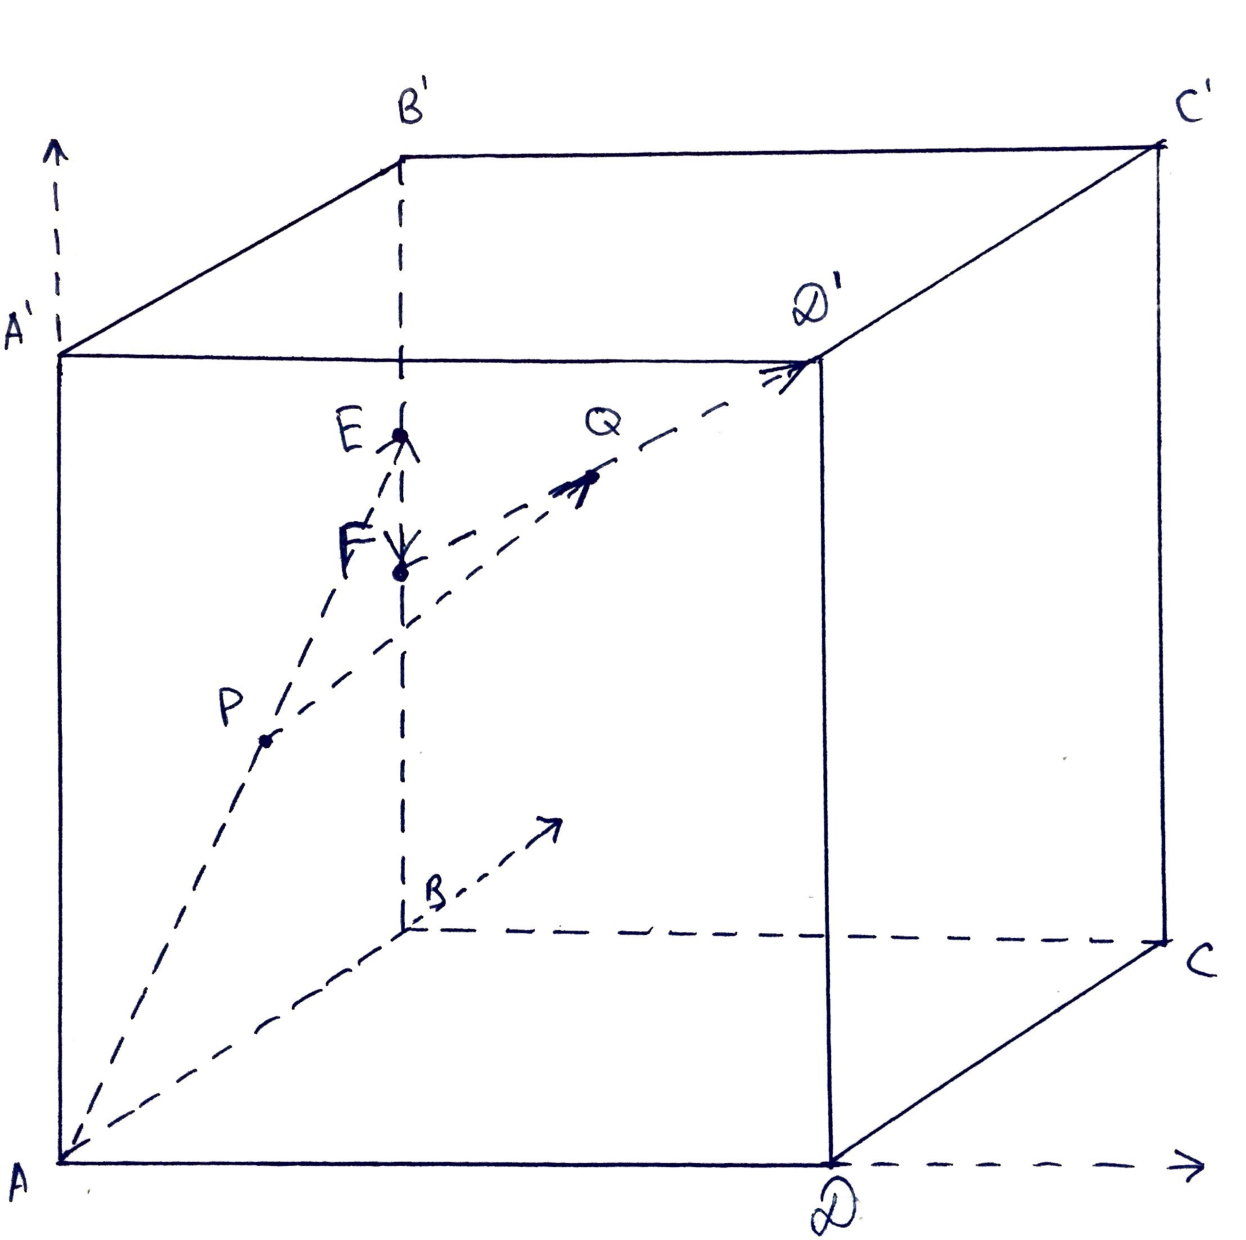
\includegraphics[width=100mm]{picture.pdf}
\end{minipage} \hfill
\begin{minipage}[b]{60mm}
	Дано: \\
	$AB...C'D'$ -- куб со стороной 4;\\
	$B'F=FB$;\\
	$BE:EB'=2:1$;
	\medskip\hrule\medskip
	Найти:
	$\angle(AE,D'F)$;\\
	$\rho(AE, D'F)$.
\end{minipage}\\
\noindent \textbf{Решение.} Обозначим $\angle(AE,D'F) = \varphi$. Введем координатную ось с т.$A$ в начале координат, тогда $A(0, 0, 0), A'(0, 0, 4), B(0,4,0),\\
B'(0, 4, 4), D(4,0,0), D'(4,0,4), F(0, 4, 2), E(0, 4, \frac{8}{3})$. Отложим вектора: $\overrightarrow{AE}, \overrightarrow{EF}, \overrightarrow{FD'}, \overrightarrow{PQ}$, где $PQ$ -- общий перпендикуляр к прямым $AE$ и $FD'$(а его длина и есть искомое расстояние). Для начала найдем угол.  Для этого найдем координаты соответствующих векторов: $\overrightarrow{AE}(0, 4, \frac{8}{3}), \overrightarrow{FD'}(4, -4, 2)$. Теперь по определению косинуса:
\begin{gather*}
cos\varphi = |cos(\angle(\overrightarrow{AE}, \overrightarrow{FD'})| = \frac{|(\overrightarrow{AE},\overrightarrow{FD'})|}{|\overrightarrow{AE}|\cdot |\overrightarrow{FD'}|} = \frac{\frac{32}{3}}{\frac{4\sqrt{13}}{3}\cdot 6} = \frac{4}{3\sqrt{13}}.\\
\varphi = arccos\frac{4}{3\sqrt{13}}
\end{gather*}
Теперь найдем длину. Заметим, что $\overrightarrow{PQ} = x\cdot \overrightarrow{AE} + \overrightarrow{EF} + y \cdot \overrightarrow{FD'}$, где $x, y$ -- неизвестные скаляры. Но мы знаем про $\overrightarrow{PQ}$, что он ортогонален и $\overrightarrow{AE}$, и $\overrightarrow{FD'}$. Следовательно, составим:
$$
\begin{cases}
	(\overrightarrow{PQ}, \overrightarrow{AE}) = 0\\
	(\overrightarrow{PQ}, \overrightarrow{FD'}) = 0
\end{cases} \Leftrightarrow
\begin{cases}
	x \cdot |\overrightarrow{AE}|^2 + (\overrightarrow{EF}, \overrightarrow{AE}) + y\cdot (\overrightarrow{AE}, \overrightarrow{FD'}) = 0 \\
	y \cdot |\overrightarrow{FD'}|^2 + (\overrightarrow{EF}, \overrightarrow{FD}) + x\cdot (\overrightarrow{AE}, \overrightarrow{FD'}) = 0 
\end{cases}
$$
Заметим, что $\overrightarrow{EF}(0, 0, -\frac{2}{3})$. Подставим в нашу систему и найдем $x, y$:
$$
\begin{cases}
	\frac{208}{9}x - \frac{16}{9} - \frac{32}{3}y = 0\\
	6y - \frac{4}{3}-\frac{32}{3}x = 0 
\end{cases} \Rightarrow
\begin{cases}
	x = 1\\y = 2
\end{cases}
$$
Таким образом, $\overrightarrow{PQ} = \overrightarrow{AE} + \overrightarrow{EF} + 2\overrightarrow{FD'}$ и $\overrightarrow{PQ}(8, -4, 4)$. Следовательно, $\rho(AE, D'F) = |\overrightarrow{PQ}| = 4\sqrt{6}$\\










\end{spacing}

\end{document}